\section{Estimator Design}

\subsection{Centralized Control Design}
Based on \cite{mellinger2013trajectory}, the controller separates position and attitude tracking. Position and velocity errors define commanded acceleration $\mathbf{\ddot{r}}_{cmd}$:

\begin{equation}
    \mathbf{e}_p = \mathbf{r}_{des} - \mathbf{r}, \quad \mathbf{e}_v = \mathbf{\dot{r}}_{des} - \mathbf{\dot{r}},
\end{equation}

\begin{equation}\mathbf{\ddot{r}}_{cmd} = K_p \mathbf{e}_p + K_d \mathbf{e}_v + \mathbf{\ddot{r}}_{\text{ff}}.
\end{equation}

Desired roll ($\phi^{des}$), pitch ($\theta^{des}$), and total thrust ($F_B^{des}$) are extracted via small-angle approximation:

\begin{equation}
    \begin{split}
        \phi^{des} &= \frac{1}{g} (\ddot{r}^{des}_{x} \sin \psi_T - \ddot{r}^{des}_{y} \cos \psi_T), \\
        \theta^{des} &= \frac{1}{g} (\ddot{r}^{des}_{y} \cos \psi_T + \ddot{r}^{des}_{y} \sin \psi_T), \\
        F_B^{des} &= m(\ddot{r}^{des}_{z} + g).
    \end{split}
\end{equation}

Inner-loop desired moments $\mathbf{M}_B^{des}$ regulate orientation against angular velocities $(p, q, r)$:

\begin{equation}
    \begin{split}        
        M_{xB}^{des} &= k_{p, \phi} (\phi^{des} - \phi) + k_{d, \phi} (p^{des} - p), \\
        M_{yB}^{des} &= k_{p, \theta} (\theta^{des} - \theta) + k_{d, \theta} (q^{des} - q), \\
        M_{zB}^{des} &= k_{p, \psi} (\psi^{des} - \psi) + k_{d, \psi} (r^{des} - r).
    \end{split}
\end{equation}

\subsection{PINN Architecture}
To address the 6-DOF rigid-body dynamics, our PINN framework utilizes continuous time $t$ as the sole independent variable to solve the time-dependent ODEs \cite{lakshminarayana_application_2022, mojgani_kolmogorov_2023, raissi_physics-informed_2019}. The neural network architecture comprises two fully connected hidden layers, each containing 64 neurons. These intermediate layers map to a 12-neuron output layer designed to predict the full kinematic state vector of the composite body, which is explicitly defined in the subsequent section. The complete network topology is illustrated in Fig. \ref{fig:pinns_architecture}.

\begin{figure}[htbp] 
    \centering 
    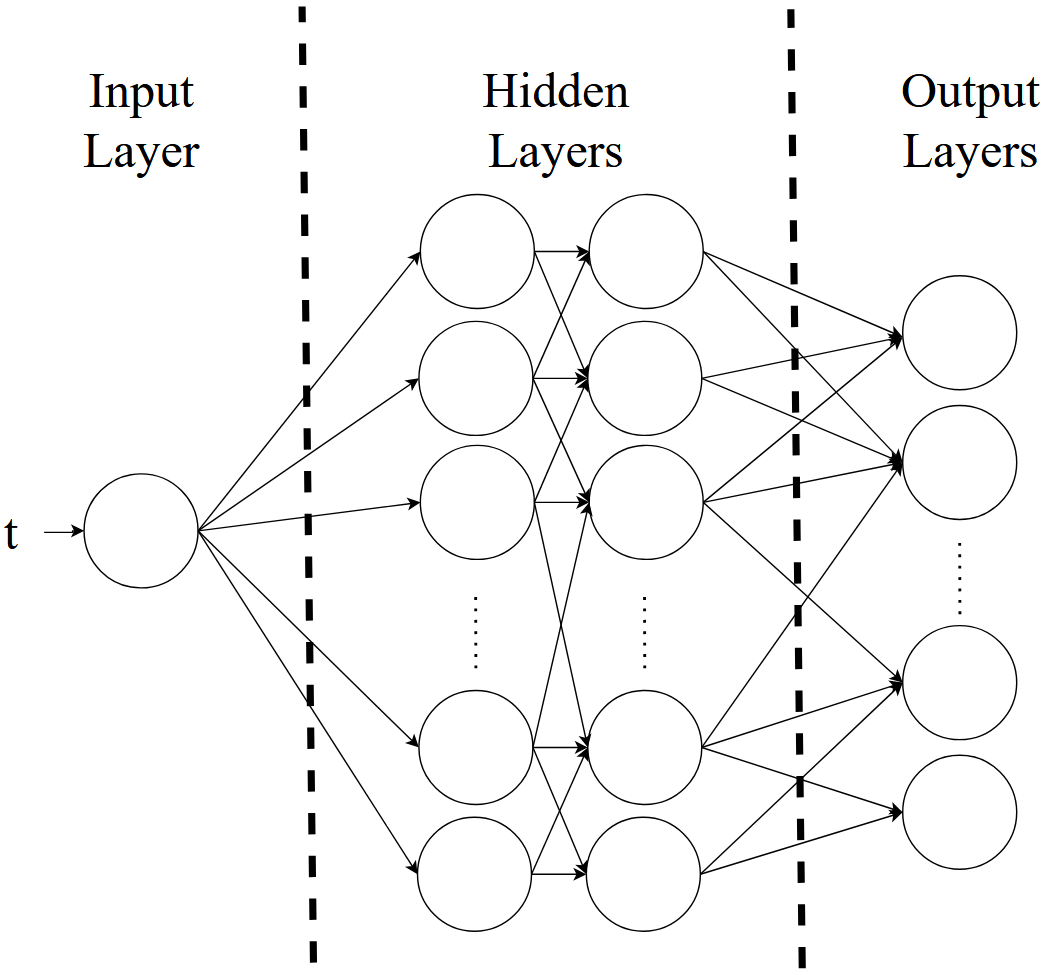
\includegraphics[width=0.3\textwidth]{images/pinns_architecture.png} 
    \caption{The proposed PINN architecture based on a fully connected ANN. The input layer accepts continuous time $t$, which is propagated through two hidden layers comprising 64 neurons each. The output layer yields the 12-dimensional kinematic state vector of the composite body defined in Eq. (\ref{eq:body_state}). A hyperbolic tangent ($\tanh$) activation function is employed across all hidden layers.}
    \label{fig:pinns_architecture} 
\end{figure}

\subsection{Loss Function Formulation}

The neural network acts as a surrogate model mapping continuous time $t$ to the predicted 6-DOF kinematic state of the system. We define the complete state vector $\mathbf{s}$, comprising the position, linear velocity, attitude, and angular velocity:

\begin{equation}
    \mathbf{s} = [\mathbf{r}^T, \mathbf{\dot{r}}^T, \boldsymbol{\eta}^T, \boldsymbol{\omega}^T]^T \label{eq:body_state}.
\end{equation}

To train the network, we formulate a composite loss function $\mathcal{L}_{total}$ \cite{serrano_physics-informed_2024, raissi_physics-informed_2019} that simultaneously penalizes empirical data deviations and violations of rigid-body dynamics. This objective function is defined as a weighted sum of the data-driven observation loss ($\mathcal{L}_{data}$), the translational physics residual ($\mathcal{L}_{trans}$), and the rotational physics residual ($\mathcal{L}_{rot}$):

\begin{equation}
    \mathcal{L}_{total} = \lambda_{1} \mathcal{L}_{data} + \lambda_{2} \mathcal{L}_{trans} + \lambda_{3} \mathcal{L}_{rot} \label{eq:loss_function}.
\end{equation}

where the hyperparameters $\lambda_{1}, \lambda_{2},$ and $\lambda_{3}$ balance the gradient contributions of each loss term.

The data loss ensures the network's predictions anchor to the physical reality measured by the onboard sensors. It is computed as the Mean Squared Error (MSE) over a temporal window of $N$ collocation points:

\begin{equation}
    \mathcal{L}_{data} = \frac{1}{N} \sum_{i=1}^{N} \left\lVert \mathbf{\hat{S}}_i - \mathbf{S}_{true,i} \right\rVert^2 \label{eq:data_loss}.
\end{equation}

To enforce the translational physical constraints, we formulate a residual loss based on the Euler-Lagrange equations \cite{haghighatdoost_euler_2026}. Let $L = T_{trans} - V$ denote the system Lagrangian, where $T_{trans}$ is the kinetic energy and $V$ is the potential energy. The translational dynamics must satisfy:

\begin{equation}
    \frac{d}{dt} \left( \frac{\partial L}{\partial \mathbf{v}} \right) - \frac{\partial L}{\partial \mathbf{r}} = \mathbf{F}_{ext}.
\end{equation}

Evaluating the kinetic inertial term yields $m\mathbf{\dot{v}}$. Rather than analytically deriving the potential gradient, we leverage PyTorch's Automatic Differentiation (Autograd) engine to dynamically compute $\frac{\partial V}{\partial \mathbf{r}}$ during the forward pass. The resulting translational physics loss minimizes the residual of these forces across the temporal window:

\begin{equation}
    \mathcal{L}_{trans} = \frac{1}{N} \sum_{i=1}^{N} \left\lVert m \mathbf{\dot{v}}_i + \frac{\partial V}{\partial \mathbf{r}_i} - \mathbf{F}_{ext, i} \right\rVert^2 \label{eq:trans_loss}.
\end{equation}

While translational dynamics are straightforward, evaluating rotational dynamics using minimal coordinates (e.g., Euler angles) introduces mathematical singularities, commonly known as gimbal lock, at extreme pitch or roll angles. To ensure global mathematical validity, we evaluate the rotational dynamics directly on the Special Orthogonal group, $SO(3)$. The rotational kinetic energy of the rigid multi-agent system is defined as

\begin{equation}
    T_{rot} = \frac{1}{2} \boldsymbol{\omega}^T \mathbf{J} \boldsymbol{\omega},
\end{equation}

\noindent where $\mathbf{J} \in \mathbb{R}^{3 \times 3}$ is the estimated inertia tensor. By applying the Lagrange-d'Alembert principle to the $SO(3)$ manifold, we obtain the coordinate-free Euler-Poincaré equations:

\begin{equation}
    \frac{d}{dt} \left( \frac{\partial T_{rot}}{\partial \boldsymbol{\omega}} \right) + \boldsymbol{\omega} \times \frac{\partial T_{rot}}{\partial \boldsymbol{\omega}} = \boldsymbol{\tau}_{ext} \label{eq:euler_poincare}.
\end{equation}

The partial derivative $\frac{\partial T_{rot}}{\partial \boldsymbol{\omega}} = \mathbf{J} \boldsymbol{\omega}$ represents the system's angular momentum, Eq. (\ref{eq:euler_poincare}) resolves into the Newton-Euler formulation for rigid body rotation. In our cooperative framework, the total external torque $\boldsymbol{\tau}_{ext}$ comprises the known applied control wrench $\boldsymbol{\tau}_{app}$ and the unknown disturbance torque $\boldsymbol{\tau}_{dist}$ generated by the payload's CoG offset. The rotational physics residual evaluated during the forward pass is thus formulated as:

\begin{equation}
    \mathcal{R}_{rot} = \left( \mathbf{\hat{J}} \mathbf{\dot{\hat{\boldsymbol{\omega}}}} + \boldsymbol{\hat{\omega}} \times (\mathbf{\hat{J}} \boldsymbol{\hat{\omega}}) \right) - \left( \boldsymbol{\tau}_{app} - \boldsymbol{\tau}_{dist} \right).
\end{equation}

Finally, the rotational loss penalizes the mean squared error of this residual, forcing the neural network to implicitly map the physical discrepancies to the true disturbance parameters:

\begin{equation}
    \mathcal{L}_{rot} = \frac{1}{N} \sum_{i=1}^{N} \left\lVert \mathcal{R}_{rot, i} \right\rVert^2 \label{eq:rot_loss}.
\end{equation}